The following figures were obtained using the procedure described previously.

In the images, we can observe certain interesting aspects, starting with Fig.~\ref{fig:noRashba}.
The image presents two graphs that illustrate the transmission coefficient ($T$) as a function of $V_b$ (in meV) and $k_0$ (in \AA$^{-1}$) for a fixed value of $\xi = (1, 0)$.
The left graph is a three-dimensional visualization where $T$ is on the $z$-axis, $V_b$ on the $x$-axis, and $k_0$ on the $y$-axis, with a color scale that varies from dark purple (lower $T$) to bright yellow (higher $T$).
The right graph is a two-dimensional heat map that offers a top view, with the $x$-axis representing $k_0$ and the $y$-axis representing $V_b$, using the same color map as the 3D graph.
Both graphs show that the transmission coefficient generally remains very close to 1, indicating high transmission.
As $V_b$ increases, $T$ tends to decrease, while the dependence on $k_0$ is minimal.
In general, the graphs demonstrate how $T$ changes with variations in $V_b$ and $k_0$, highlighting a slight decrease in $T$ as $V_b$ increases and an insignificant change with respect to $k_0$.

This result shows a contradiction with what is already specified in the literature, as in graphene, total transmission would be expected due to the material's inherent properties\cite{horsell2008, Young2009}.

\begin{figure}%[!ht]
    \centering
   % \begin{minipage}[t]{0.48\textwidth}
        %\centering
        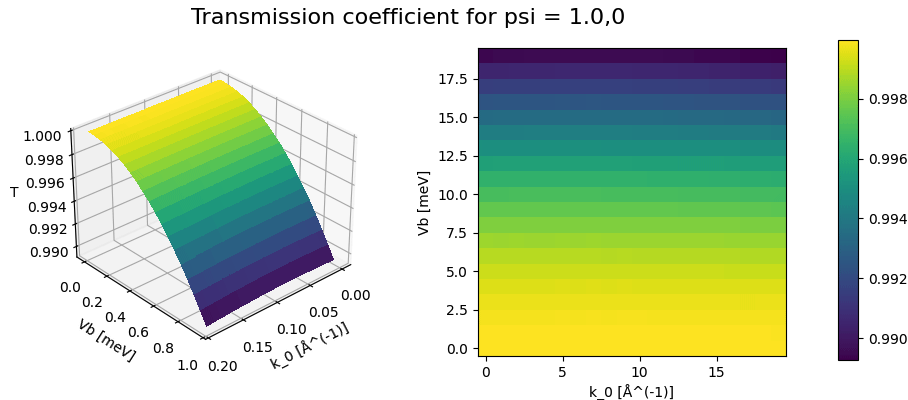
\includegraphics[width=0.88\textwidth]
        {../assets/images/No-Rashba/TCoefficient(1.0,0)xalpha=0beta=0}
        \caption{Transmission coefficient ($T$) in pristine graphene with initial pseudospinor configuration $\xi = (1, 0)$, plotted against potential barrier height ($V_b$, in meV) and initial wave vector ($k_0$, in \AA$^{-1}$). The 3D plot and 2D heatmap show that transmission is largely independent of the initial wave vector but decreases slightly as the barrier height increases (from ~1 to ~0.990).}
        \label{fig:noRashba}
   % \end{minipage}
    \end{figure}
   %\hfill

These observed differences can be primarily attributed to the following aspects related to our method and simulation conditions:

\begin{itemize}
    \item Wave Packet Characteristics:
    Our simulation uses a wave packet (GWP) composed of multiple momentum eigenstates instead of considering a single eigenstate.
    This choice implies simultaneous contributions from several states, potentially generating quantum interferences that slightly affect the transmission coefficient\cite{Staelens2021}.
    This point, highlighted by our time-dynamic modeling, marks a significant difference compared to ideal theoretical models where such interferences do not appear.

    Additionally, our simulation explicitly considers the time variable, something uncommon in previous ideal and static theoretical studies.
    Investigating how these dynamic aspects, such as phase time or tunneling time, specifically affect the observed transmission is an important objective proposed for future work.

    \item Quantum interference effects due to packet dispersion over time:
    As suggested in the literature\cite{MolgadoMex2018}, when a sufficiently wide Gaussian wave packet evolves temporally, it disperses spatially in such a way that different parts of it simultaneously interact with the barrier, causing internal interferences with itself.
    Such interference is a possible additional cause of the fluctuations in transmission observed in our numerical results.
\end{itemize}
    
\begin{figure}%[!ht]    
   % \begin{minipage}[t]{0.48\textwidth}
        \centering
        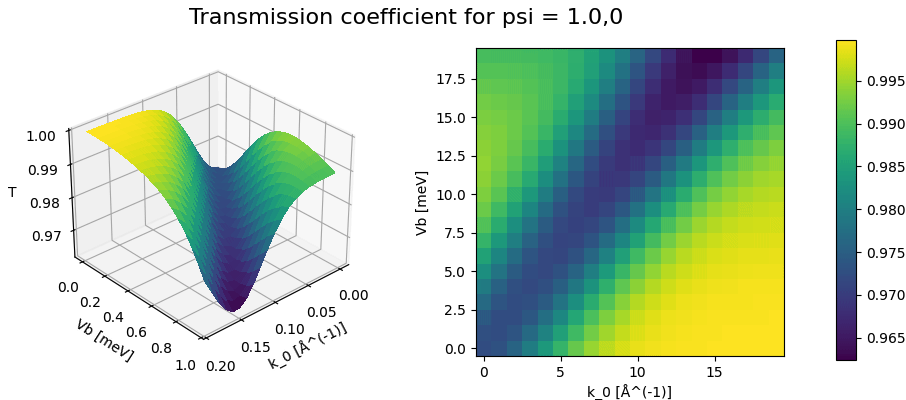
\includegraphics[width=0.88\textwidth]{../assets/images/Rashba/TCoefficient(1.0,0)xalpha=0.2beta=-0.2}
        \caption{Transmission coefficient ($T$) versus potential barrier height ($V_b$) and initial wave number ($k_0$) for an initial pseudospinor configuration $\xi = (1, 0)$. The 3D surface and 2D colormap reveal a non-monotonic dependence on $V_b$ and $k_0$, highlighting the influence of spin–orbit coupling on transmission through the barrier.}
        \label{fig:rashba}
   % \end{minipage}
\end{figure}

These points clearly explain the differences found from a methodological perspective and link our numerical results to the theoretical prediction mentioned in previous studies.
This not only clarifies the apparent contradiction but also clearly reinforces the connection between our specific results and the main objective of analyzing dynamic effects and properties that arise when using Gaussian wave packets in quantum tunneling simulations in graphene-based systems.

On the other hand, we have the transmission under the presence of SOIR (Fig.\ref{fig:rashba}).

A correlation between the variables is observed: generally, with greater potential barrier height ($V_b$) and greater initial wave number ($k_0$), lower transmission is expected.
However, the spin-orbit interaction introduces more complex behavior.
As $k_0$ increases and $V_b$ decreases, the transmission approaches 1, indicating a higher probability of quantum tunneling due to SOIR\@.

Although the variation in the transmission coefficient is small (on the order of $10^{-2}$), it is significant and attributable to the SOIR interaction.

The electrons, with their different pseudospin components, interact, and this interaction is affected by the initial wave number of the Gaussian wave packet (GWP), as observed in previous studies\cite{Serna2019}.
Therefore, SOIR modulates the interaction, which in turn causes the fluctuations observed in the transmission coefficient.

It is important to highlight here that the expression for the current vector used in our analysis (Eq. \ref{eq:componentes}) follows directly from the standard Dirac–Rashba Hamiltonian for graphene and has been reported in related contexts\cite{AvishaiPhysRevB2021}.
In this work, we leverage that established expression to (i) decompose the current into pseudospinorial components and (ii) quantify cross-correlations induced by the Rashba interaction, which jointly enable a clear interpretation of the numerical trends observed in our time-dependent wave-packet simulations.
Thus, the role of Eq. \ref{eq:componentes} here is not to introduce a new formula, but to provide a rigorous and practical framework for dissecting the transmission variations and their spinorial origin\cite{Serna2019}, thereby informing future theoretical and experimental studies on spintronic transport in graphene.

Finally, we stress a modeling limitation and its remedy: the canonical Dirac–Rashba term is neglected in the pristine case because its magnitude is typically very small in graphene.
If the experimental platform realizes a giant Rashba coupling via proximity or adatoms (e.g., graphene on TMDs or with Au), the canonical term must be included explicitly.
In that regime, the wave-packet propagation is expected to exhibit stronger spin-dependent splitting and precession, altered resonance conditions, and potentially a crossover between Klein and anti-Klein tunneling\cite{DellAnnaJPhysCondMatt2018, AvsarNatCommun2014, WangPhysRevX2016}.
Our numerical framework readily accommodates this extension by upgrading to a four-component spinor and adding the Dirac–Rashba operator to the Hamiltonian.


After thoroughly analyzing the numerical results and discussing the particular aspects observed in the electronic transmission coefficients with and without Rashba interaction, we can synthesize below the main conclusions reached in this work, highlighting their theoretical and technological implications, as well as the perspectives for future studies and applications.
